\maketitle


\section{Predicting Bike Station Occupancy}
\subsection{Feature Engineering}
\subsubsection{Selection of Station}
In choosing the stations I was going to use I decided to display them on a map.
This would make it easier to choose stations which would have different behaviour.
I decided to choose station 97 (Kilmainham Gaol) as it is the furthest from the city center.
I also chose station 109 (Buckingham Street) as it is beside Connolly and I assumed it would have drastically different behaviour than my other station.

\begin{figure}[H]
\centering
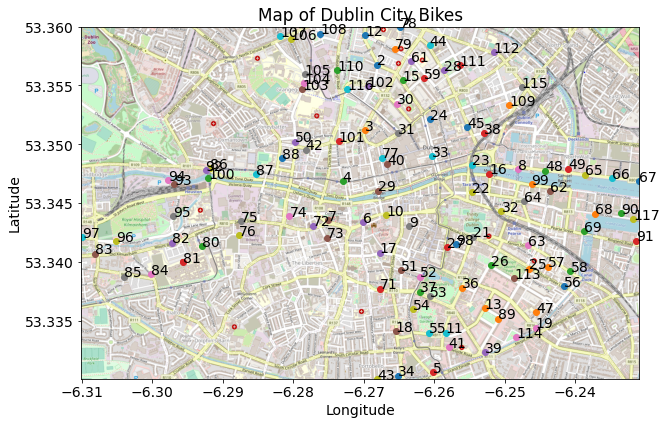
\includegraphics[width=0.5\textwidth]{images/map.png}
\caption{Map of Dublin Bike stations.}
\end{figure}




\begin{figure}[H]
    \centering
    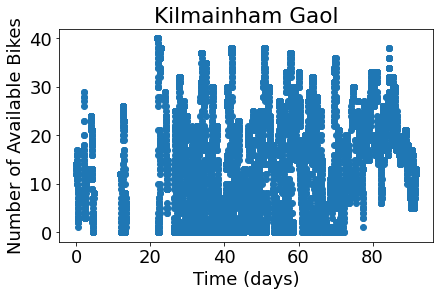
\includegraphics[width=0.5\textwidth]{images/kilmainham data.png}
    \caption{Map of Dublin Bike stations.}
    \end{figure}
\par 

\begin{figure}[H]
    \centering
    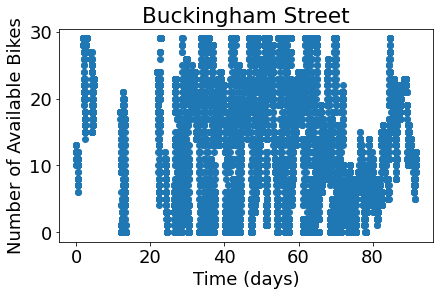
\includegraphics[width=0.5\textwidth]{images/buckingham data.png}
    \caption{Map of Dublin Bike stations.}
    \end{figure}

\subsubsection{Data Cleaning}
As can be seen in figures 2 and 3, much of the data in the first few weeks is missing.
I decided to simply remove the first 27 days in both datasets as 
there was so much missing that it would likely make it more difficult to 
work with the data in a way that didn't negatively affect the performance of the models.
It is likely that there were other missing data points, this is evident in that not every day has the same number of entries (between 287 and 289).
This is unlikey to have any major impact on my predictions as it is very close to 288
(the number of 5 minute time blocks in a day).

\subsubsection{Feature Selection}
The features I took from the datasets are 

\par 


\subsection{Ridge Regression}
I initially decided to use ridge regression to predict future values. 
I wanted to use some form of linear regression because I used them for a similar problem in my group project.
Lasso regression is more likely than Ridge to reduce coefficients to zero but I was curious to see how even the lightly weighted parameters were affected so I decided to use ridge regression instead.
\par 

I used 5 fold cross validation to find the ideal value for alpha to use and I found that varying alpha had very little effect until alpha became quite large 
as can be seen in figures\dots. 
I decided to use a value of 1 for every model as this value gave a near minimum mean-squared error for every prediction model.
\par 
The metric I used to evaluate performance is mean squared error. 
I feel that this is a suitable metric as it tells us how far off predictions from a model are. 

\par 



\subsection{K Neighbours Regression}

\subsection{Evaluation}
\subsubsection{Method 1}
\subsubsection{Method 2}
